\section{Model}
\label{ch:method}
\noindent	

This chapter will discuss the model used to attain the goals of the project.

\subsection{System overview}

\begin{figure}[H]
	\begin{center}
		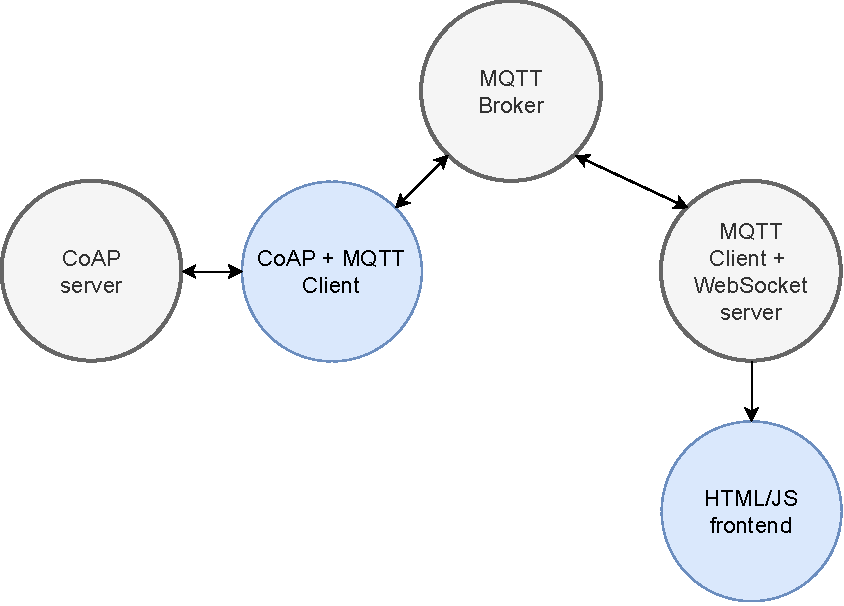
\includegraphics[width=\textwidth]{./doc/system}
		\caption{Overview of the system}
		\label{system-overview}
	\end{center}
\end{figure}

Figure~\ref{system-overview} shows a brief overview of the different components in the system. They are as follows:

\begin{itemize}
	\item \textit{CoAP server} A CoAP server responsible for providing current CPU and memory usage. This component should ideally symbolise some sort of IoT device which is of interest to monitor.
	\item \textit{CoAP + MQTT Client} This component is responsible for picking up on MQTT based requests for curent CPU/memory usage, then translating these requests into the CoAP protocol and sending them to the CoAP server. Upon recieving a response from the CoAP server, this response is then translated back into a message able to be published to the MQTT broker.
	\item \textit{MQTT Broker} The MQTT broker is responsible for managing all publications and subscriptions authored by the two MQTT clients. If either of the two clients wish to subscribe to a topic, this subscription will be registered and remembered by the broker. The next time a client wishes to publish something to this topic, this publication is retransmitted to all clients currently subscribed to this topic.
	\item \textit{MQTT Client + WebSocket server} This component works as a bridge between the MQTT broker and the end user frontend. It is meant to regularly publish requests for current CPU/memory utilization and subscribe to the topic in which the responses to these requests are published. Upon receiving a response, it is then translated into a WebSocket message which is sent to the frontend. This component should also be able to benchmark the RTT between publishing a request and receiving a response, to later enrich the message sent to the frontend with the measured time.
	\item \textit{HTML/JS frontend} The frontend is a comparatively rather simple component, all things considered. It listens for published messages from the WebSocket server and updates three different graphs which plot CPU usage, memory usage and round trip time as a function of time. The frontend is not capable of sending messages in and of itself, but instead relies on the WebSocket server being able to pump out new information.
\end{itemize}

\iffalse
With regards to C- and D-level diploma work, it is insufficient to merely perform a practical construction or programming project. A systematic study must also be carried out, e.g. an evaluation and analysis of the design or program. The study should result in objective facts, preferably in the form of tables and diagrams, into which your own conclusions are built in. The study can be a verification of a design that meets the requirement specification, or a comparison of competing alternatives. It is acceptable to allow users to answer a questionnaire or be interviewed. It is also possible to evaluate web-pages and other user interfaces according to usability criteria.

The method section is the point at which your chosen method and intended procedure during the research are discussed. This section shall not be a chronological diary filled with irrelevant details, but should contain information given in such a way that it is understandable for the reader and enables him/her to interpret your results and repeat your work, i.e. in order to check the results. Here, the tools, assumptions, mathematical models, performance measures and assessment criteria are presented. It is also at this point that the means adopted for the evaluation and verification of the computer programs and technical solution proposals are presented. This can include a test plan to check that the structure works and criteria to assess its usefulness. In research reports regarding natural science and technology this chapter is often called “Model”, “System Model” or “Simulation Model”.

Justify your choice of methodology/model. This choice is very important, because it could be the actual key to the result of your research. Comment on the method's possible weaknesses and problems that may arise during actual implementation. Refer to the problem wording in the introduction chapter. It is possible, for example, to write “problem P1 is attempted through the method M1 and problem P2 through…” 

In your report, you should - depending on what the report is about- find information about what you have investigated and how you have gathered and processed data. Possible questionnaires, interview questions and the likes can be presented as appendices. Detailed descriptions concerning experimental formats of possible interest to those wanting to repeat the experiment should also be included in this chapter.
\fi
